\documentclass[12pt,a4paper,oneside]{report}

% ============================================================
% Packages
% ============================================================
\usepackage[T1]{fontenc}
\usepackage{tgtermes}          % Times New Roman equivalent (TeX Gyre Termes)
\usepackage{amsmath,amssymb}
\usepackage{parskip}
\usepackage{graphicx}
\usepackage{xcolor}
\usepackage[a4paper,margin=1in]{geometry}
\usepackage{longtable,booktabs,array}
\usepackage{setspace}
\usepackage{listings}
\usepackage{float}

% Chapter/Section formatting (from DKU template)
\usepackage{titlesec}
\titleformat{\chapter}[display]
  {\bfseries\huge}
  {\Large \chaptertitlename\ \thechapter}
  {2ex}
  {\titlerule
   \vspace{1ex}%
   \filright\MakeUppercase}
  [\vspace{1ex}%
\titlerule]
\titleformat{\section}{\normalfont\Large\bfseries}{\thesection}{1em}{}
\titleformat{\subsection}{\normalfont\large\bfseries}{\thesubsection}{1em}{}
\titleformat{\subsubsection}{\normalfont\normalsize\bfseries}{\thesubsubsection}{1em}{}

% Bibliography
\usepackage[style=numeric-comp, url=false]{biblatex}
\addbibresource{bibfile.bib}

\usepackage{upquote}
\usepackage[allcolors=blue,colorlinks=true]{hyperref}
\usepackage{xurl}
\usepackage{microtype}
\usepackage{bookmark}
\usepackage{calc}
\usepackage{etoolbox}
\usepackage{subcaption}

\newcommand{\instructions}[1]{{\color{black}\itshape #1}}

\urlstyle{same}
\doublespacing
\graphicspath{{figures/}}

% Code listing style
\lstdefinestyle{diffstyle}{
  basicstyle=\ttfamily\small,
  frame=single,
  breaklines=true,
  columns=fullflexible,
  keepspaces=true
}

% ============================================================
% Metadata
% ============================================================

\newcommand{\authorname}{Jiahe (Jay) Chen}
\newcommand{\thetitle}{Diff-Eval: An AI-Driven Agentic Workflow for Code Quality Evaluation}
\newcommand{\submissiondate}{May 2026}
\newcommand{\mentor}{Jiacheng Shen}
\newcommand{\academicunit}{Division of Natural and Applied Sciences}
\newcommand{\mentortitle}{Assistant Professor of Electrical and Computer Engineering}

% ============================================================
\begin{document}

% About Majors at DKU
\instructions{Background:  Duke Kunshan University (DKU) is an interdisciplinary institution that grants dual undergraduate degrees, an MOE Chinese degree and a degree from Duke University in Durham, United States. The principal structure of DKU majors is robustly interdisciplinary. No student confines their study to a single discipline (for example, biology or economics). Instead, all students engage in broad inquiry related to a subject or question (for example, political economy or global health) and take a wide variety of courses related to that area (for example, in public policy, history, ethics, or economics). As a result, our graduates are prepared to engage in a wide variety of inquiries using multiple methodologies to address complex issues that require interdisciplinary approaches.
This has implications for our vision and expectations of undergraduate theses and design projects, which reflect this broad interdisciplinary training. At DKU, every student completes a two-year project known as signature work which consists of multiple interconnected parts including thematic courses, experiential learning, capstones, and a final product. It seeks to integrate students' interdisciplinary educational experience and culminates in the creation of a product in a scholarly, creative, or applied nature in leu of an undergraduate thesis or design required by JED. Because DKU encourages students to cultivate their independence and creativity as one of its institutional student learning outcomes, the student-led signature work projects often reflect students' own particular interdisciplinary interests and training.  In addition, signature work has an intensive emphasis on problem-solving and skill-development which is much needed for any interdisciplinary inquiry; thus, students' final products are evidence of transferrable skills that students have acquired and demonstrated through the 2-year program, rather than content knowledge narrowly defined by disciplinary training.
In sum, while the Chinese major declared with any given student might be construed narrowly, the experience of our students is much broader---and intentionally so.  This is a distinctive feature of our curriculum, and this distinctiveness results in broadly interdisciplinary submissions from our graduates' submitting theses or design projects. We have designed this to prepare our students for a wide variety of graduate programs in China and the West, where interdisciplinary training is a competitive advantage.}

% ============================================================
% Title Page
% ============================================================
\begin{titlepage}

\vspace*{\bigskipamount}

\begin{center}
{\sffamily\LARGE\bfseries\MakeUppercase\thetitle\par}

\bigskip

by

\bigskip

{\Large \authorname}

\bigskip

Class of 2026

Computation and Design (Computer Science)

\bigskip

Signature Work Product, in partial fulfillment of the \\
Duke Kunshan University Undergraduate Degree Program

\bigskip

\emph{\submissiondate}

\bigskip

Signature Work Program \\
Duke Kunshan University

\end{center}

\vfill

\textbf{\textsf{APPROVALS}}

\bigskip\bigskip\bigskip
\hrule

Mentor: \mentor, \mentortitle, \academicunit

\bigskip\bigskip\bigskip
\hrule

\end{titlepage}

% ============================================================
% Front Matter
% ============================================================
\clearpage
\pagenumbering{roman}

\setcounter{tocdepth}{1}
\tableofcontents

% ---- Acknowledgements ----
\chapter*{Acknowledgements}
\label{acknowledgements}
\addcontentsline{toc}{chapter}{Acknowledgements}

Doing signature work was a bittersweet journey, mixed with excitement and disappointment. I remember the sadness when finding out the experiment results didn't improve by even a single percent after spending a whole night working on it. But I also remember the surprise when new methods finally worked out and broke our best accuracy records.

During this period of time, the encouragement of my mentor, Jiacheng Shen, was like a silver light that motivated me to keep going. Looking back, I cannot imagine how I could have gotten here without his support. He provided topic inspiration, research methodology guidance, execution priorities, and networks to help this experiment succeed. Jiacheng had regular meetings with me to make sure the experiment was on the right track. When there were urgent issues to deal with, he even spent his personal time to help. I sincerely appreciate his time and dedication to this project. The outcome of this project is not only a paper or a diploma, but also lifelong gains in my critical thinking, academic literacy, and information retrieval ability. Your advising helped me a lot!

I would also like to express my gratitude to my parents, who financially supported me in attending DKU. Without their sponsorship, I would not even have had the opportunity to start this journey.

Thanks again to Jiacheng and my parents.

\newpage

% ---- Abstract ----
\chapter*{Abstract}
\addcontentsline{toc}{chapter}{Abstract}

Code quality is a critical concern in software engineering, directly affecting system stability, maintainability, and development efficiency. Traditional static analysis tools detect only syntactic and structural issues through rule-based pattern matching, falling short on design-level defects such as SOLID violations that require understanding architectural intent. LLM-based analysis offers richer semantic understanding, but sending proprietary codebases to cloud APIs introduces data leakage and compliance risks that are unacceptable in many enterprise and government settings. This work proposes that, in the context of code quality evaluation, \textbf{Small LLM + Agentic Workflow $\approx$ Full-Size LLM}---delivering near-cloud accuracy entirely on local hardware with zero data egress.

This work proposes \textbf{Diff Eval}, a workflow-driven approach that simulates real software development scenarios---attempting to extend the code under test---to assess extensibility and surface design defects through the resulting code diff.

Evaluated on a benchmark dataset of 240 code examples (48 per principle, spanning Python, Java, Kotlin, and C\#, across three difficulty levels), Diff Eval achieves \textbf{87.92\%} accuracy using a local Qwen3.5 9B model via Ollama---significantly outperforming single-agent (70.00\%) and two-agent (55.83\%) baselines, closing approximately 70\% of the performance gap to a full-size cloud LLM (95.83\%), and running entirely on-premise with zero data egress. Accuracy remains robust across code complexity levels, enabled by a context-compression mechanism that insulates the system from long-code noise.

\vspace{1em}
\noindent\textbf{Keywords:} \textbf{Software engineering}, \textbf{LLM}, \textbf{code quality}, \textbf{design principles}, \textbf{agentic workflow}

% ---- List of Figures & Tables ----
\addcontentsline{toc}{chapter}{List of Figures}
\setcounter{tocdepth}{1}
\listoffigures\newpage

\addcontentsline{toc}{chapter}{List of Tables}
\setcounter{tocdepth}{1}
\listoftables\newpage

% ============================================================
% Main Matter
% ============================================================
\clearpage
\pagenumbering{arabic}

% ============================================================
\chapter{Introduction}
\label{ch:introduction}
% ============================================================

Software design quality is a critical concern in modern software engineering. While syntactic errors and surface-level bugs can be caught by compilers and static analyzers, \emph{design-level} defects---violations of principles like SOLID~\cite{Martin2000, Martin2017}---remain notoriously difficult to detect automatically. These violations degrade maintainability, increase coupling, and raise the cost of future modifications~\cite{Sharma2018, Palomba2015}.

Recent advances in large language models (LLMs) have opened new possibilities for code understanding~\cite{Fan2023}. However, directly prompting an LLM to judge whether a code snippet violates a design principle yields poor results---even with optimized prompt strategies, accuracy remains limited and varies dramatically across principles~\cite{Pehlivan2025}. Meanwhile, agentic multi-model workflows have shown promise for related tasks like test smell detection~\cite{Melo2025}, suggesting that workflow design matters as much as model capability.

A practical constraint motivates fully local deployment. Enterprise and government codebases routinely contain proprietary or regulated information that cannot be transmitted to external cloud APIs without risk of data leakage or compliance violation. Regulatory frameworks such as the EU AI Act~\cite{EUAIAct2024} and national security auditing criteria such as Katakri 2020~\cite{Katakri2020} impose strict data-residency and access-control requirements on organisations handling sensitive data. Research on cloud computing privacy further highlights systemic risks of data outsourcing---including insider threats, unauthorised access, and loss of organisational control over sensitive assets~\cite{Ghorbel2017}. These pressures from both industry and academia motivate a code-quality analysis system that runs entirely on-premise with zero data egress.

This work proposes a fundamentally different approach grounded in a core hypothesis: \textbf{simulating code extension reveals design defects more effectively than asking a model to judge code quality directly}. When a developer tries to extend poorly designed code, the design flaws surface as forced, wide-ranging modifications to existing logic. By observing the diff that results from such a simulated extension, a system can detect design violations through objective evidence rather than subjective LLM assessment.

The \textbf{Diff Eval} workflow operationalizes this principle through five parallel detection channels, one per SOLID principle. Each channel generates a principle-specific extension scenario, modifies the code accordingly, computes a unified diff, and checks whether the diff pattern matches a known violation signal. A final ranking step aggregates results across all five channels.

The contributions of this work are:
\begin{enumerate}
  \item A \textbf{diff-based detection methodology} that converts subtle structural violations into concrete, observable diff patterns---making them tractable for small LLMs.
  \item A \textbf{context-compression mechanism} (the Pre-Verification stage) that isolates the diff signal from full source context, enabling robust detection across code of varying complexity.
  \item A \textbf{fully local, privacy-preserving} system that demonstrates a core principle: \textbf{Small LLM + Agentic Workflow $\approx$ Full-Size LLM}. Diff Eval on a local 9B model achieves 87.92\% accuracy, closing approximately 70\% of the performance gap between a plain small-model baseline (70.00\%) and a full-size cloud LLM (95.83\%), while running entirely on consumer hardware with zero data egress.
\end{enumerate}

% ============================================================
\chapter{Background}
\label{ch:background}
% ============================================================

\section{SOLID Principles}

The SOLID principles, formulated by Robert C. Martin~\cite{Martin2000}, are five design guidelines for object-oriented software:

\begin{itemize}
  \item \textbf{SRP} (Single Responsibility Principle): A class should have only one reason to change.
  \item \textbf{OCP} (Open/Closed Principle): Software entities should be open for extension but closed for modification.
  \item \textbf{LSP} (Liskov Substitution Principle): Subtypes must be substitutable for their base types without altering program correctness.
  \item \textbf{ISP} (Interface Segregation Principle): Clients should not be forced to depend on interfaces they do not use.
  \item \textbf{DIP} (Dependency Inversion Principle): High-level modules should depend on abstractions, not concrete implementations.
\end{itemize}

Violations of these principles lead to rigid, fragile, and tightly coupled code that resists modification~\cite{Martin2017, AlOmar2023}.

\section{Traditional Code Quality Evaluation}

Traditional code quality evaluation relies on static analysis tools (SonarQube, Checkstyle, PMD) and metric-based approaches (CBO, RFC, LCOM~\cite{AlOmar2023}). Static analyzers apply rule-based pattern matching and are fast, but detect only syntactic and structural issues; design-level defects like SOLID violations require understanding \emph{intent} and \emph{architectural context} that rules cannot capture~\cite{Sharma2018}. Metric-based approaches quantify structural properties but cannot identify \emph{which} principle is violated or \emph{why}. ML classifiers~\cite{Palomba2015} can detect subtler patterns but require large labeled corpora and do not generalize across languages without retraining. These limitations motivate LLM-based approaches, which learn code semantics from large corpora and generalize across languages without per-language engineering.

\section{LLM-Based SOLID Violation Detection}

Pehlivan et al.~\cite{Pehlivan2025} conduct the first systematic empirical study on prompting LLMs to detect SOLID violations, evaluating CodeLlama 70B, DeepSeek-Coder 33B, Qwen2.5-Coder 32B, and GPT-4o-mini on a 240-example benchmark under four prompt strategies. The few-shot (\texttt{example}) strategy consistently performs best; GPT-4o-mini peaks at 69.2\% and Qwen2.5-Coder 32B at 53.8\%, while both open-source models stay below 25\%. The Qwen family's strong showing at fewer parameters motivates our choice of Qwen for local inference.

\paragraph{Violation-type breakdown.}
Figure~\ref{fig:pehlivan_f1_model} disaggregates results by principle. \textbf{DIP is essentially unsolved}: F1 ranges from 0.0 (CodeLlama 70B) to just 10.8 (Qwen2.5-Coder 32B). ISP is highly variable (13.6--71.1), while SRP is the most tractable (55.6--99.7). Model scale does not predict principle-level performance---CodeLlama 70B underperforms GPT-4o-mini on every principle despite its larger size.

\paragraph{Difficulty degradation.}
Figure~\ref{fig:pehlivan_acc_level} shows accuracy by difficulty level averaged across models. SRP holds at 77.7\% through Moderate but drops to 40.2\% at Hard; OCP degrades from 64.8\% to 18.0\%; DIP is near-zero at all levels (6.6\% / 0.4\% / 0.4\%). Two classes emerge: \emph{surface-visible} principles (SRP, OCP) that degrade with complexity, and \emph{structurally opaque} principles (DIP, ISP, LSP) that are unsolved regardless of difficulty. These patterns directly motivate Diff Eval: converting opaque structural violations into observable diff signals and compressing code context for robustness at Hard difficulty.

\begin{figure}[htbp]
\centering
\begin{subfigure}[t]{0.48\textwidth}
  \centering
  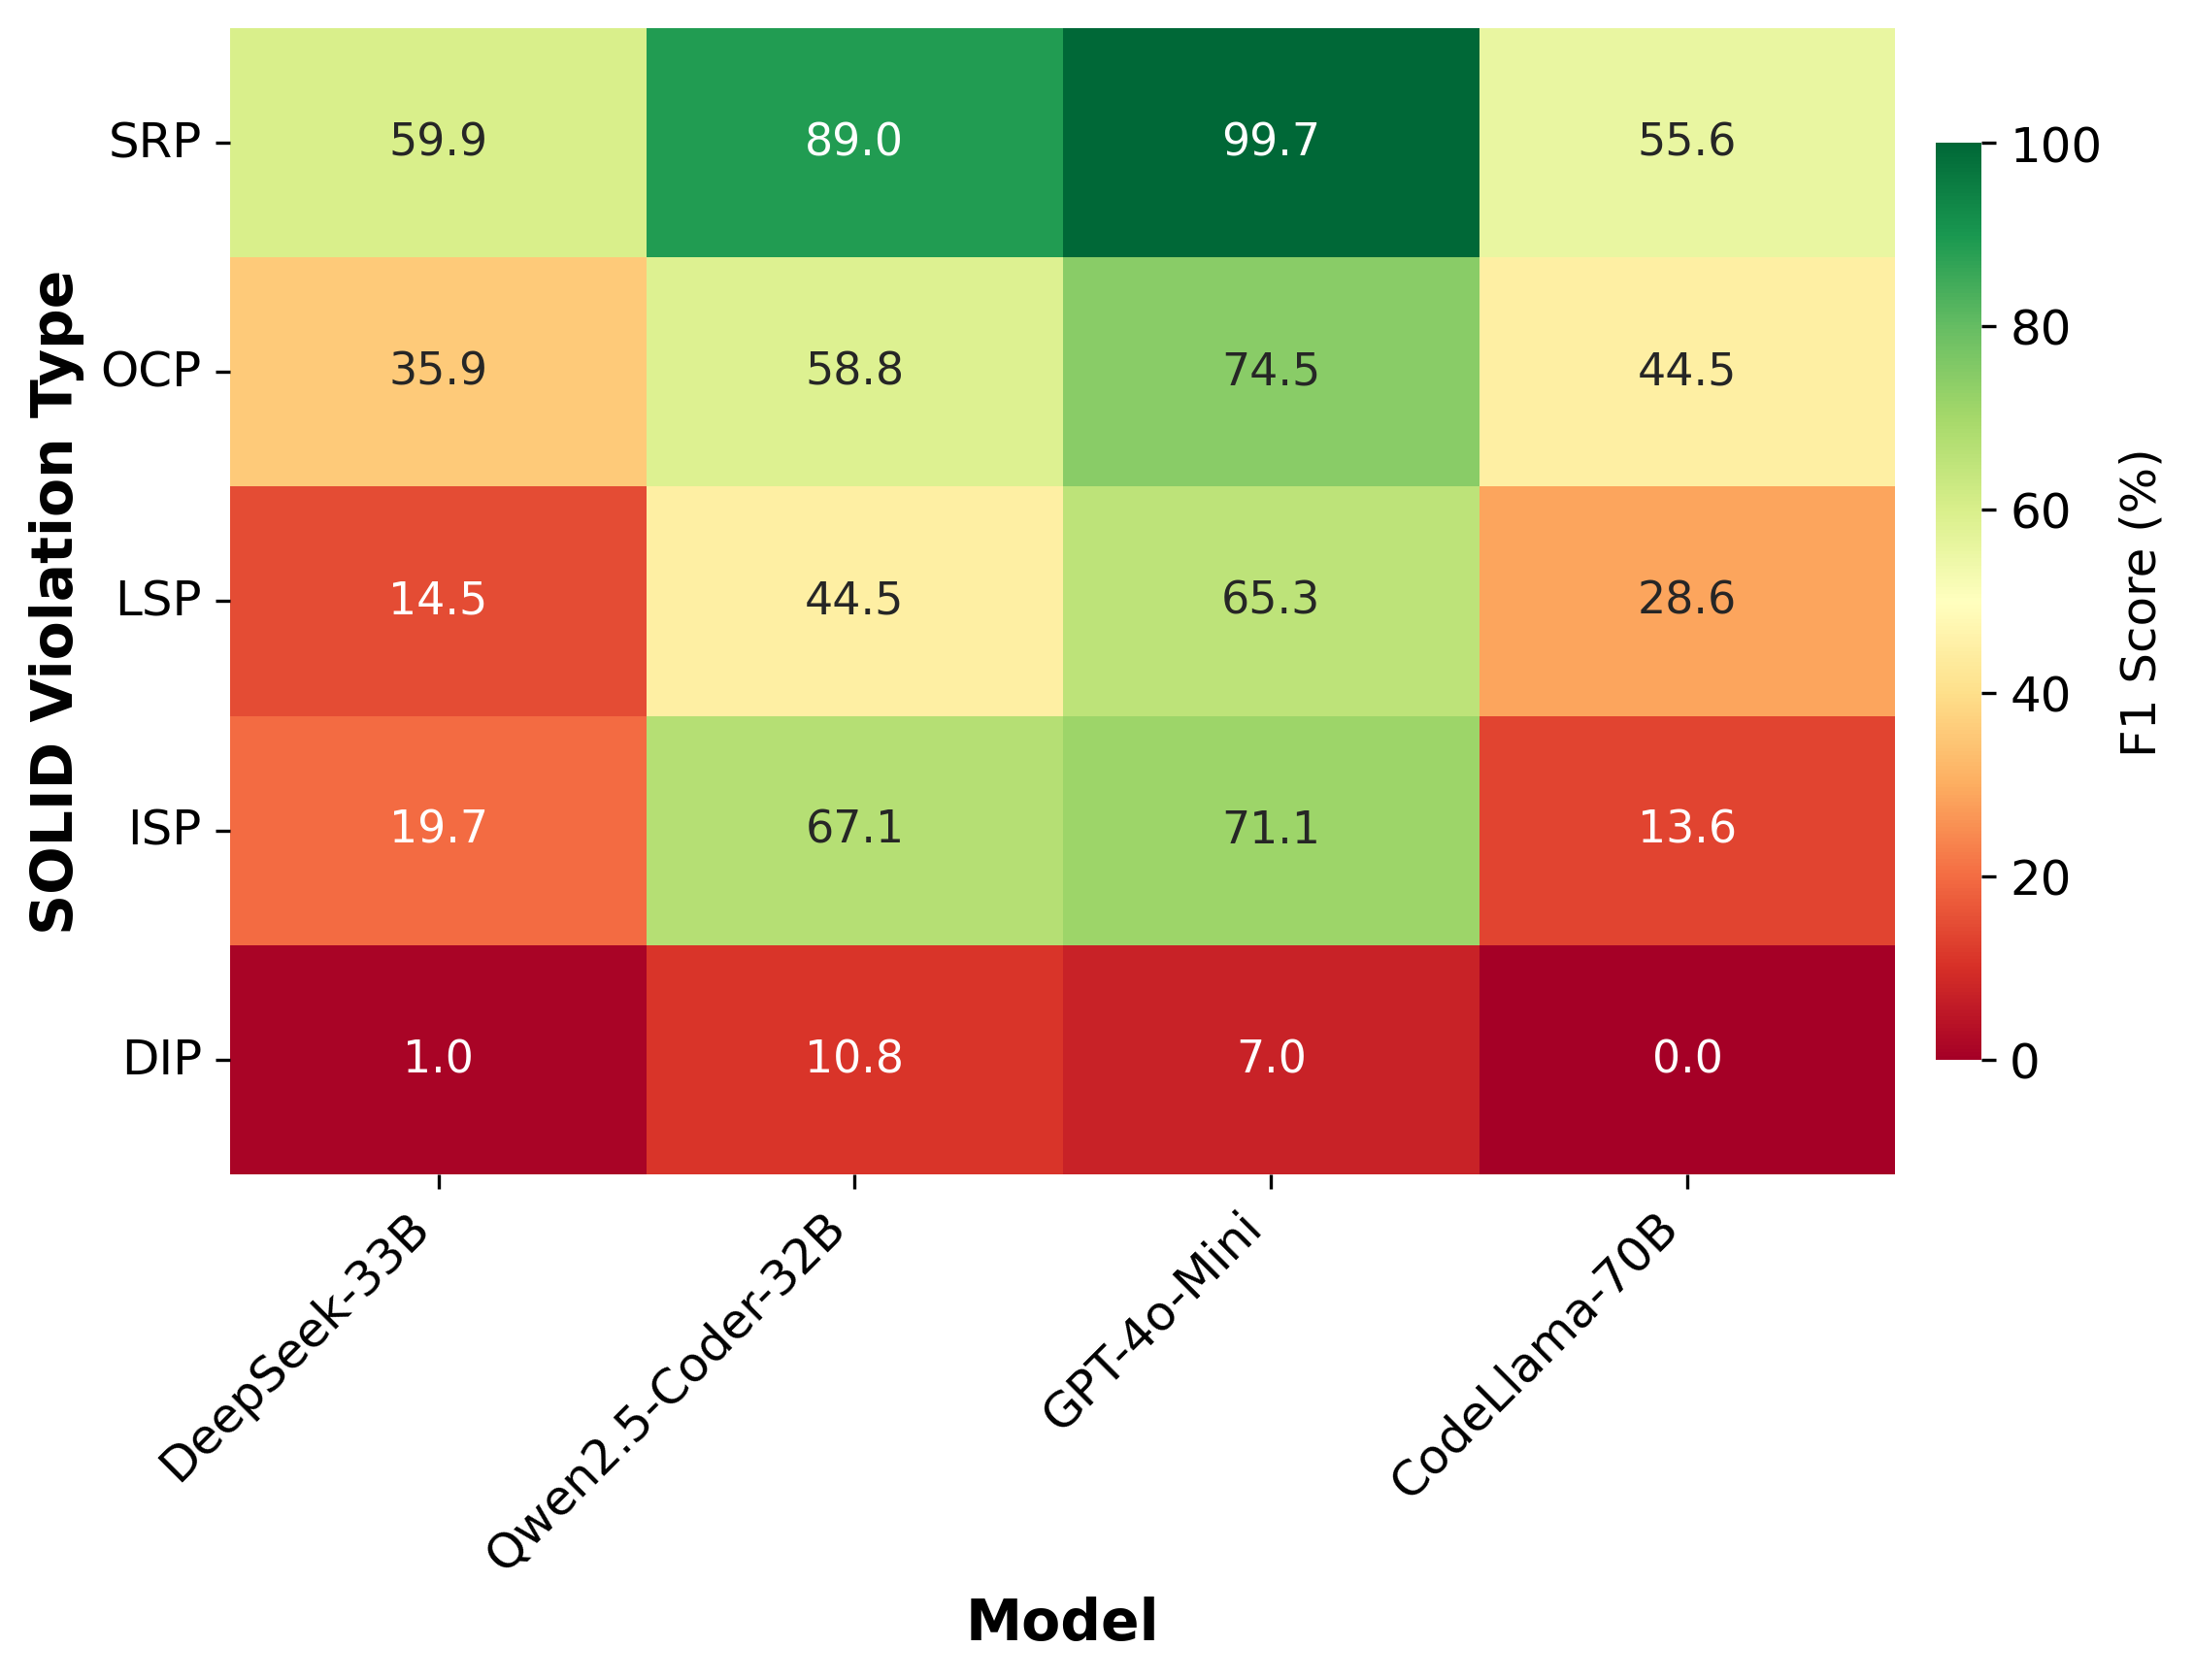
\includegraphics[width=\textwidth]{solid_violations_f1_by_model.png}
  \caption{Per-principle F1 by model. DIP is near-zero for all models.}
  \label{fig:pehlivan_f1_model}
\end{subfigure}
\hfill
\begin{subfigure}[t]{0.48\textwidth}
  \centering
  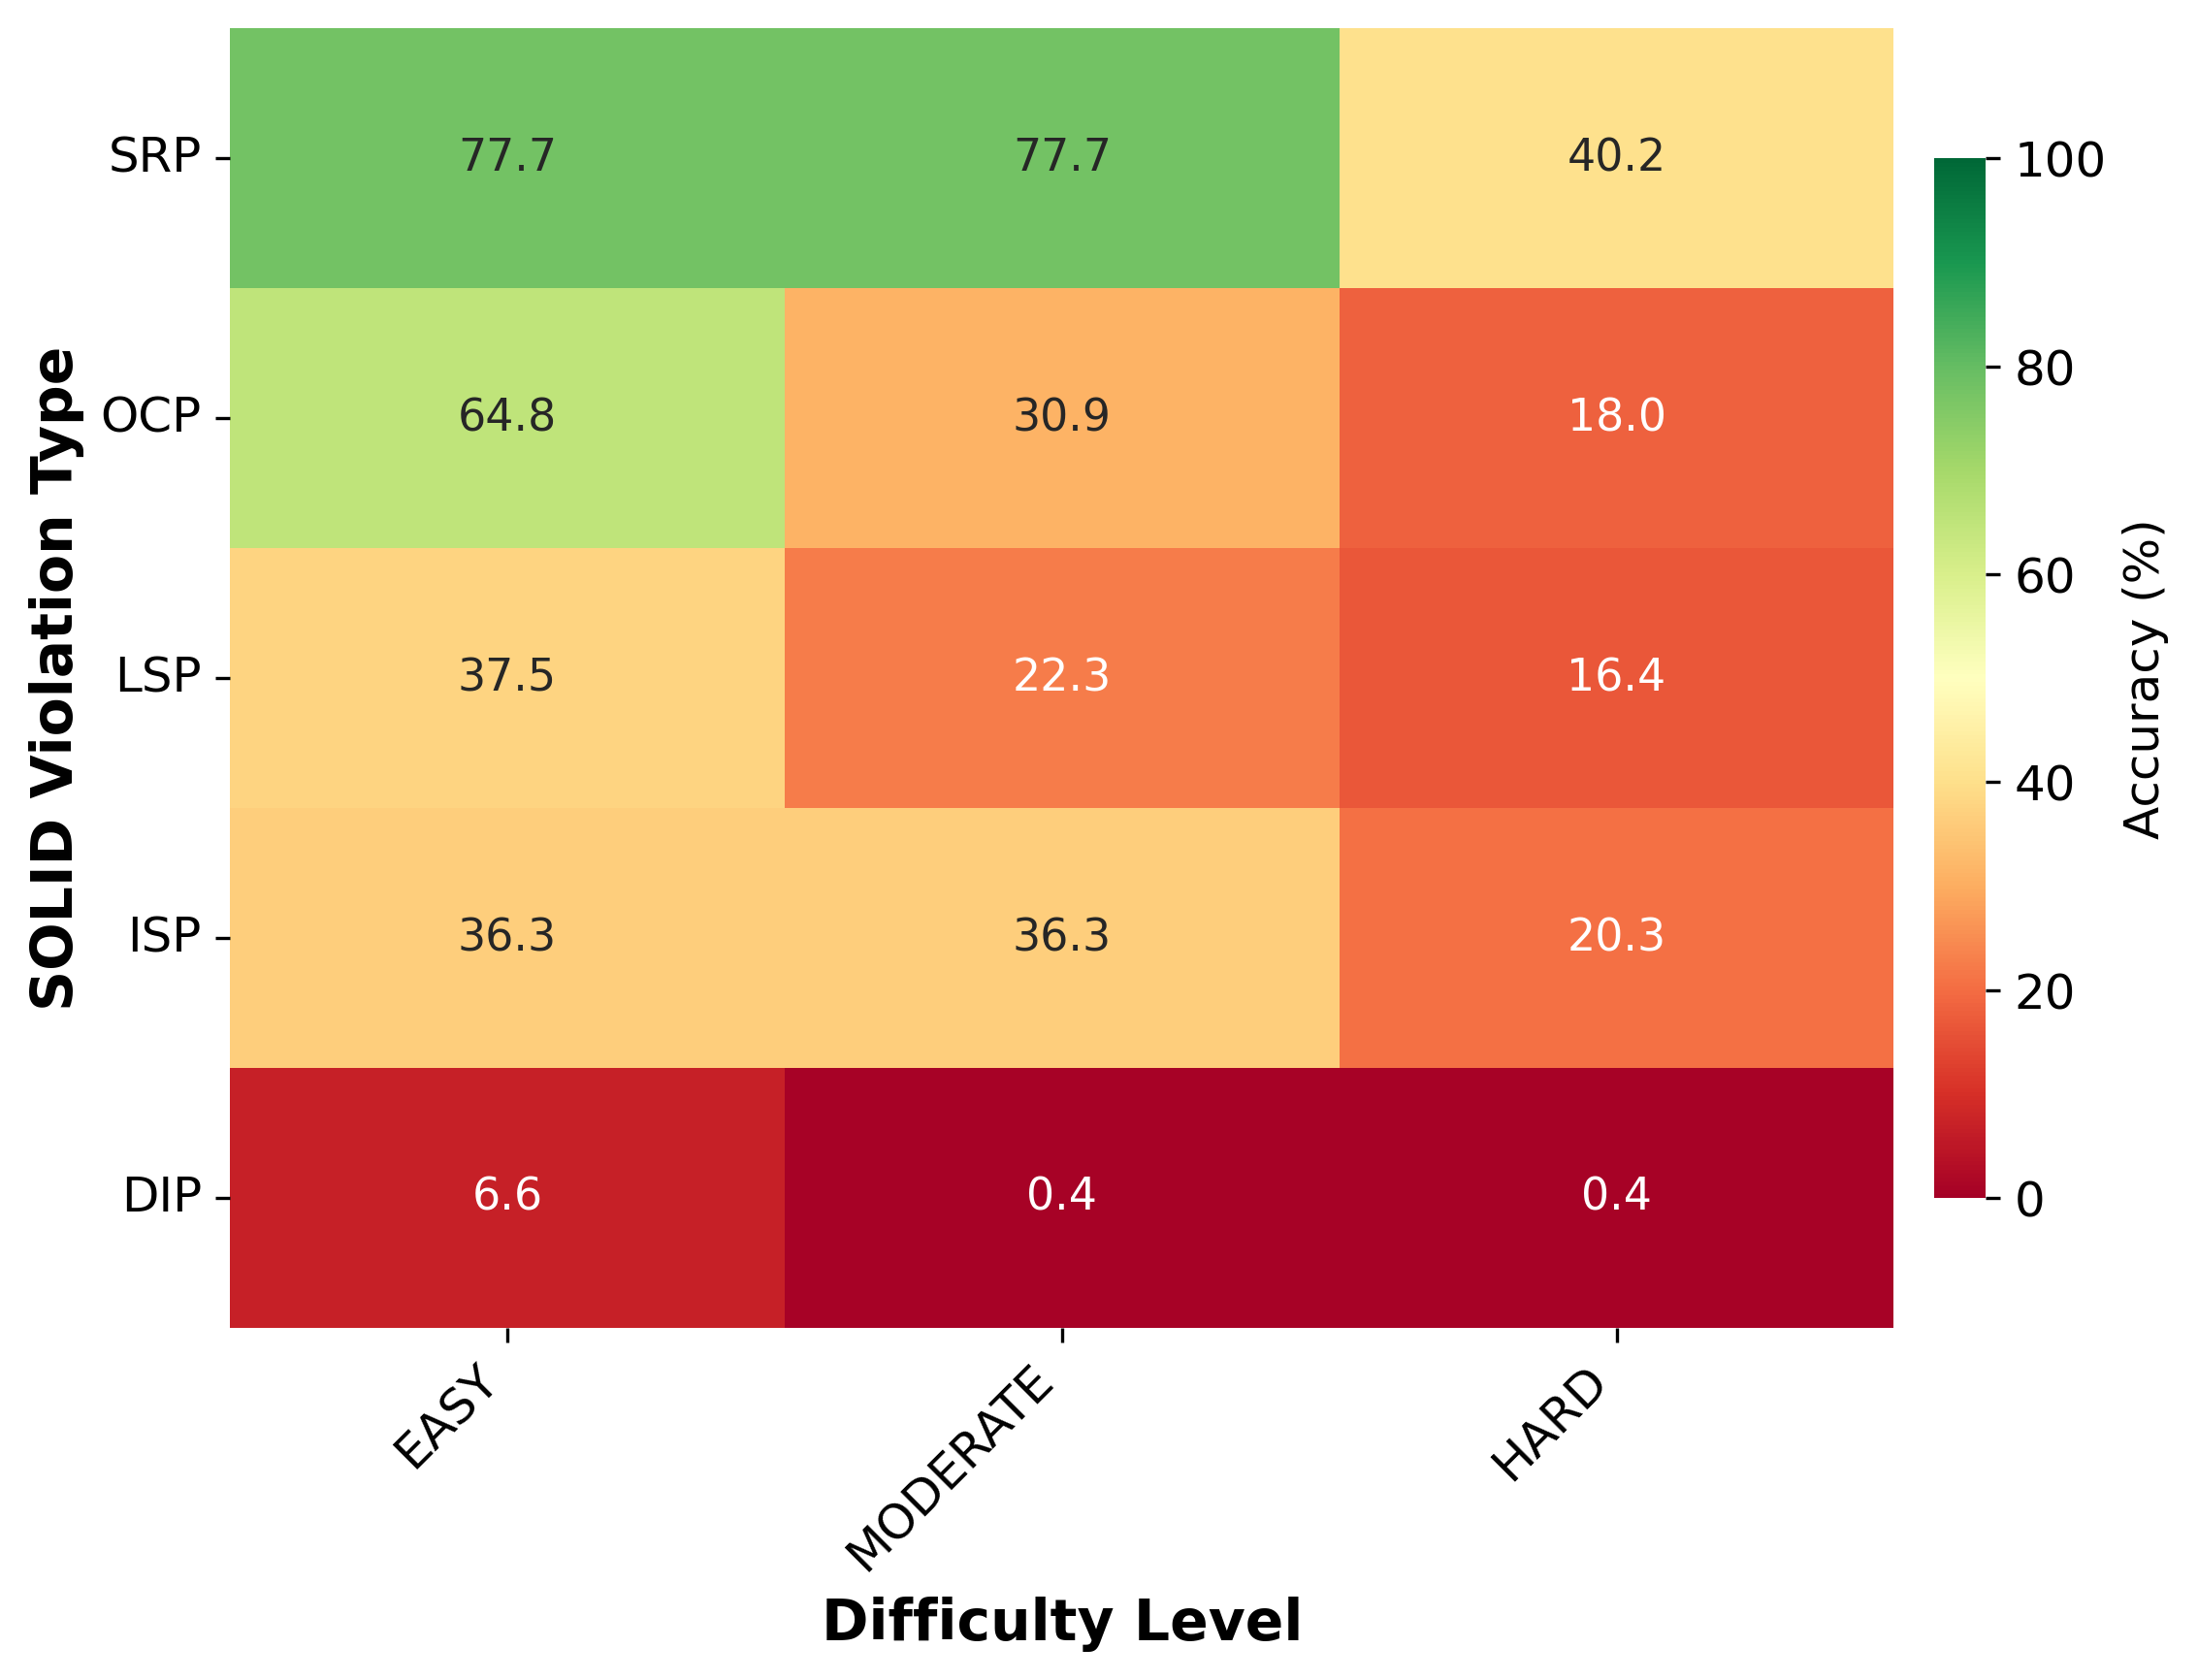
\includegraphics[width=\textwidth]{solid_violations_accuracy_by_level.png}
  \caption{Per-principle accuracy by difficulty. DIP near-zero at all levels.}
  \label{fig:pehlivan_acc_level}
\end{subfigure}
\caption{Results from Pehlivan et al.~\cite{Pehlivan2025} on the 240-example SOLID benchmark.}
\label{fig:pehlivan_combined}
\end{figure}

Our \textbf{Single Agent baseline} replicates Pehlivan et al.'s \texttt{example} strategy using Qwen3.5 9B, establishing a direct comparison point.

\section{Agentic Approaches to Code Quality}

Agentic LLM workflows---multi-step pipelines where specialized agents collaborate rather than a single model acting in isolation~\cite{Wang2024}---have shown strong results for complex reasoning tasks. Frameworks like ReAct~\cite{Yao2023} and LangGraph~\cite{LangGraph2024} provide the infrastructure for stateful, multi-actor pipelines.

Most relevant to our design, Melo et al.~\cite{Melo2025} apply agentic workflows to \emph{test smell} detection and refactoring using small models (3B--14B). They compare one-agent, two-agent (Detector + Evaluator), and four-agent configurations (Figure~\ref{fig:melo_workflow}). Their key findings: Phi-4-14B with four agents performs within 5\% of single-agent GPT-4o-mini, and the Detector--Evaluator feedback loop consistently improves detection quality over single-pass approaches.

\begin{figure}[htbp]
\centering
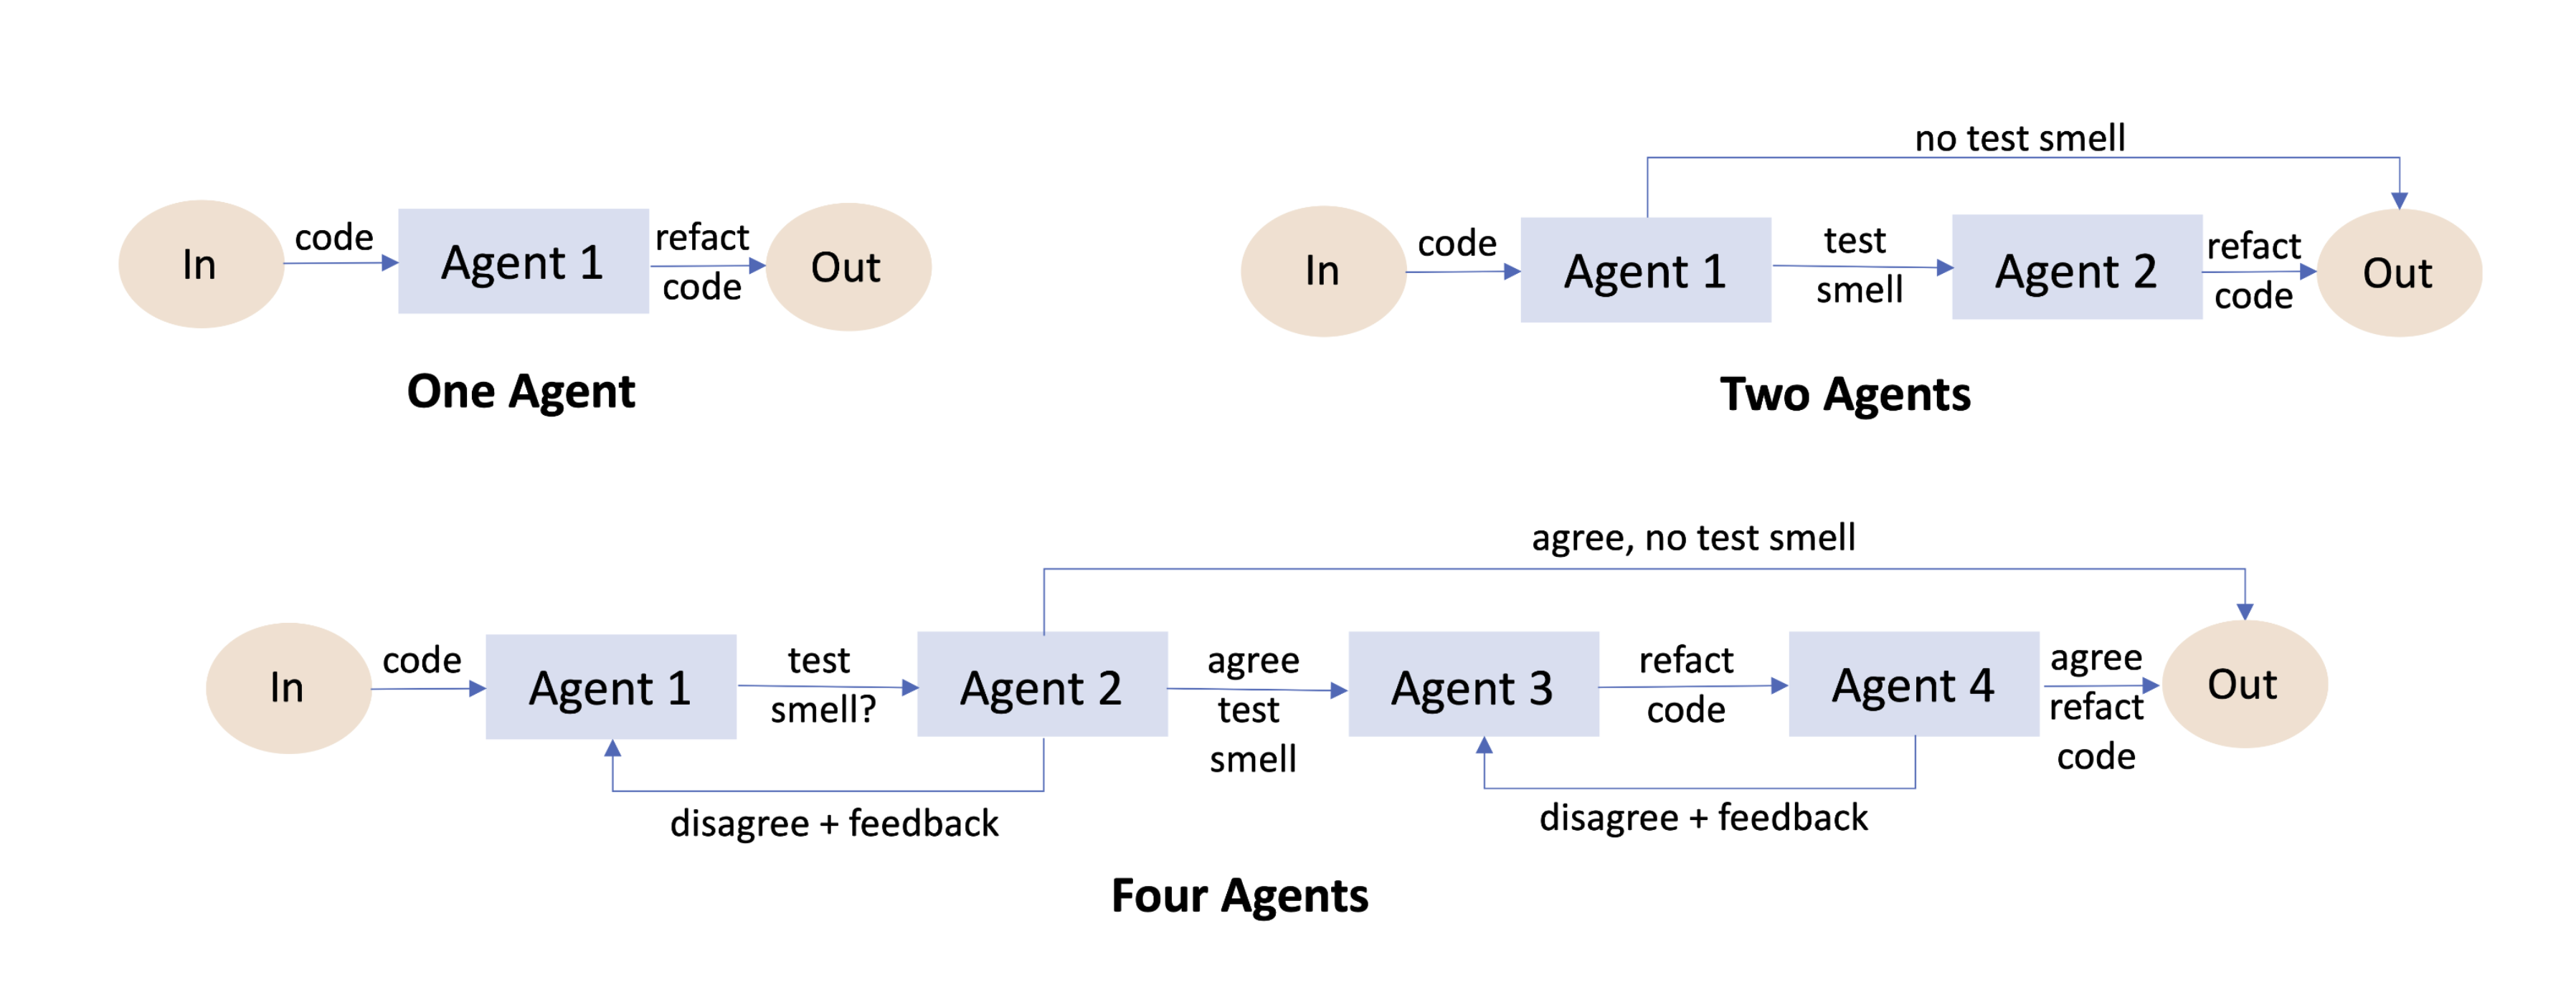
\includegraphics[width=\textwidth]{test_smell_agent.png}
\caption{One-, two-, and four-agent workflow configurations for test smell detection from Melo et al.~\cite{Melo2025}. The Detector--Evaluator pattern informs our Two-Agent baseline.}
\label{fig:melo_workflow}
\end{figure}

Our \textbf{Two-Agent baseline} directly adopts the Detector--Evaluator pattern for SOLID detection, with Agent~2 critiquing and refining Agent~1's output over up to 3 iterations. Our \textbf{Diff Eval} workflow extends this further: rather than improving judgment through iteration, it replaces static judgment with behavioral observation---generating code diffs as objective evidence of design violations.

% ============================================================
\chapter{Methodology}
\label{ch:methodology}
% ============================================================

\section{The Diff Eval Workflow}

\subsection{Core Insight: Code Extensibility as a Design Quality Signal}

The Diff Eval workflow is grounded in a fundamental property of code extensibility: \textbf{well-designed code can be extended by adding new code, while poorly designed code forces modification of existing code}. This property generalizes across all SOLID principles: each violation type manifests as a characteristic pattern of forced modifications when the code is challenged with a principle-specific extension task.

Rather than asking an LLM to abstractly judge whether code violates a design principle, Diff Eval simulates a real development scenario: it generates a realistic feature request, asks the LLM to implement it, and then examines the resulting code diff to determine what kind of changes were required. The diff provides objective, structural evidence that is far more reliable than subjective LLM judgment.

\subsection{Architecture Overview}

The system deploys five parallel detection channels---one per SOLID principle---each operating independently through four stages, followed by a Unified Ranking step that aggregates results. Figure~\ref{fig:architecture} illustrates the overall architecture.

\begin{figure}[htbp]
\centering
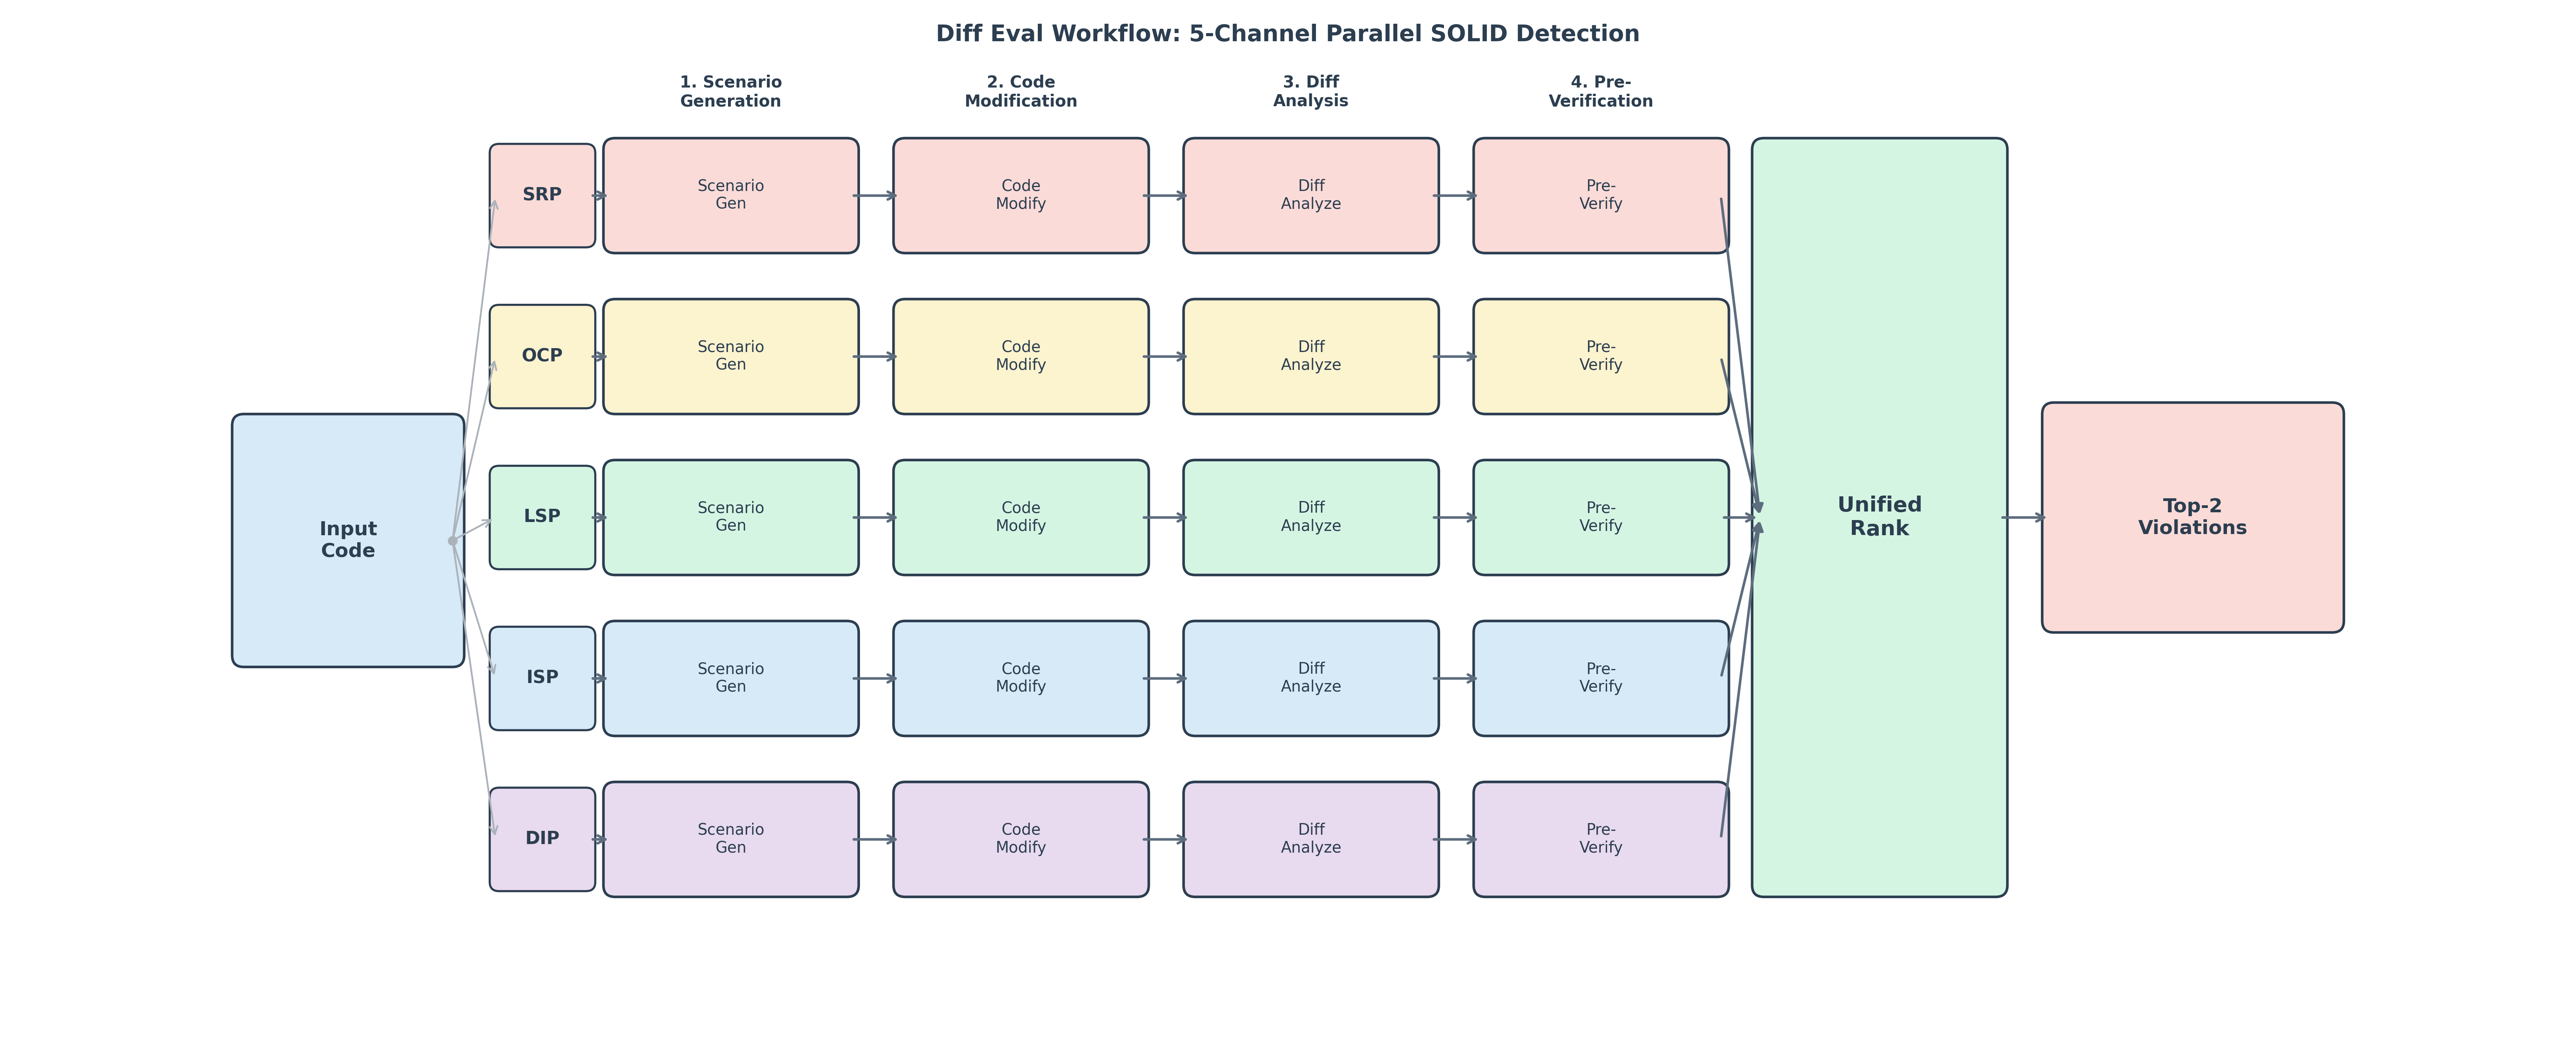
\includegraphics[width=\textwidth]{architecture_diff_eval.png}
\caption{Diff Eval system architecture: five parallel SOLID-principle channels (Scenario Generation $\to$ Code Modification $\to$ Diff Analysis $\to$ Pre-Verification) aggregated by Unified Ranking.}
\label{fig:architecture}
\end{figure}

\subsection{Stage 1: Scenario Generation}

A principle-specific prompt instructs the LLM to generate a realistic extension task tailored to surface violations of the target principle. The coupling between scenario design and signal mapping is the key innovation: each scenario is engineered so that a specific violation type produces a distinctive, recognizable diff pattern. Table~\ref{tbl:scenarios} summarises the scenario and signal for each principle.

\begin{table}[htbp]
\centering
\small
\begin{tabular}{@{}p{0.11\textwidth}p{0.38\textwidth}p{0.43\textwidth}@{}}
\toprule
\textbf{Principle} & \textbf{Scenario} & \textbf{Signal} \\
\midrule
SRP & Generate a change scoped to a single architectural layer (presentation, business, or persistence). & Modifying one layer forces edits in other layers $\Rightarrow$ mixed responsibilities. \\
\addlinespace
OCP & Generate a task requiring a new type, variant, or case to be added. & New variant requires modifying existing \texttt{if-else}/\texttt{switch} logic rather than extending via new polymorphic types. \\
\addlinespace
LSP & Create a polymorphic application exercising both parent and subclass through the same interface. & Subclass throws exceptions or alters return-value contracts, breaking the parent class contract. \\
\addlinespace
ISP & Create a new class implementing an existing interface but needing only a subset of its methods. & New class forced to provide \texttt{pass}/\texttt{NotImplementedError} stubs for unused methods $\Rightarrow$ interface too broad. \\
\addlinespace
DIP & Switch a high-level class from one concrete dependency to another without introducing abstractions. & Concrete class name changed in multiple locations inside the high-level class $\Rightarrow$ tight coupling. \\
\bottomrule
\end{tabular}
\caption{Principle-specific scenarios and diff signals used in Stage~1 of Diff Eval.}
\label{tbl:scenarios}
\end{table}

\subsection{Stage 2: Code Modification}

The LLM modifies the original code according to the generated scenario. This produces a concrete, modified version of the code that represents a realistic attempt to extend the system.

\subsection{Stage 3: Diff Analysis}

A unified diff is computed between the original and modified code. This diff is the primary evidence for violation detection---it objectively shows what changed, where changes occurred, and how extensively existing code was modified versus new code being added.

\subsection{Stage 4: Pre-Verification}

Each channel's pre-verifier applies the principle-specific signal mapping to determine whether the observed diff pattern matches the expected violation signal. The pre-verifier outputs a verdict for its assigned principle, indicating whether the violation signal is present and how clearly it is observable in the diff.

\subsection{Unified Ranking}

All five pre-verification results are aggregated by a final ranking node. This node receives all five per-principle verdicts and produces a ranked list of detected violations (Top-N), ordered by how clearly the violation signal is observable in each channel's diff.

\section{Technical Implementation}

The Diff Eval system is implemented as a LangGraph~\cite{LangGraph2024} state machine, where each node represents an LLM invocation or computation step and edges define the data flow between stages. LangGraph manages the five parallel detection channels and the final aggregation step as a single directed graph with branching and merging. The LLM interface is provided by LangChain-Ollama, bridging the workflow engine to a local Ollama~\cite{Ollama2024} inference server that serves quantized models with zero data egress; the primary model is Qwen3.5 9B~\cite{Qwen2025}. Diffs between original and modified code are computed using Python's \texttt{difflib} library. Each of the five channels uses principle-specific prompts for both scenario generation and pre-verification, with the full prompt templates available in the project repository.

\section{Baseline Methods}

Two baselines are used for comparison, each grounded in prior work:

\begin{itemize}
  \item \textbf{Single Agent}: Replicates the approach of Pehlivan et al.~\cite{Pehlivan2025}---a one-shot LLM prompt using the \texttt{example} (few-shot) strategy, which was shown to be the most effective prompt strategy for the Qwen model family. The LLM receives the code and directly outputs which SOLID principle is violated.
  \item \textbf{Two-Agent (Detector + Evaluator)}: Implements the Detector--Evaluator workflow pattern from Melo et al.~\cite{Melo2025}, adapted for SOLID detection. Agent~1 (Detector) identifies a potential violation with reasoning; Agent~2 (Evaluator) critiques the detection result and suggests corrections. The two agents iterate for up to 3 rounds until consensus is reached or the iteration limit is hit.
\end{itemize}

All three workflows (Single Agent, Two-Agent, Diff Eval) use the same underlying model (Qwen3.5 9B) to ensure that performance differences are attributable to workflow design rather than model capability.

\section{Benchmark Dataset}

The evaluation uses the benchmark dataset constructed by Pehlivan et al.~\cite{Pehlivan2025}, consisting of 240 manually validated code examples:
\begin{itemize}
  \item 48 examples per SOLID principle (SRP, OCP, LSP, ISP, DIP)
  \item 4 programming languages: Python, Java, Kotlin, C\#
  \item 3 difficulty levels: Easy (avg.\ 33 LOC), Moderate (avg.\ 140 LOC), Hard (avg.\ 306 LOC)
  \item Each example has a single known ground-truth violation
\end{itemize}

\section{Evaluation Metrics}
\label{sec:metrics}

We report the following metrics:

\textbf{Top-2 Accuracy.} The fraction of examples where the ground-truth violation appears among the model's top-2 ranked predictions:
\begin{equation}
  \text{Top-2 Accuracy} = \frac{1}{N} \sum_{i=1}^{N} \mathbf{1}[y_i \in \{\hat{y}_i^{(1)}, \hat{y}_i^{(2)}\}]
\end{equation}

In the remainder of this paper, \textbf{Accuracy} refers specifically to Top-2 accuracy. Real-world code frequently exhibits multiple design violations simultaneously; Top-2 Accuracy reflects the system's practical utility---if the correct violation appears in the top two, a developer reviewing the output will see it.

\textbf{Mean Reciprocal Rank at 2 (MRR@2).} Averages the reciprocal of the rank at which the ground-truth violation first appears (capped at rank 2):
\begin{equation}
  \text{MRR@2} = \frac{1}{N} \sum_{i=1}^{N} \frac{1}{\text{rank}_i}, \quad \text{rank}_i = \begin{cases} 1 & \text{if } \hat{y}_i^{(1)} = y_i \\ 2 & \text{if } \hat{y}_i^{(2)} = y_i \\ \infty & \text{otherwise} \end{cases}
\end{equation}

MRR@2 rewards systems that rank the correct answer higher: a perfect Top-1 system scores 1.0, while a system that always places the correct answer at rank 2 scores 0.5.

\textbf{Macro-F1.} Per-class F1 is the harmonic mean of precision and recall for each SOLID principle, where predictions are resolved from the top-2 output. Macro-F1 is the unweighted average across all five classes, treating each principle equally and penalising systems that excel on easy principles (e.g., SRP) while failing on harder ones (e.g., DIP):
\begin{equation}
  F_1^{(c)} = \frac{2 \cdot \text{Precision}^{(c)} \cdot \text{Recall}^{(c)}}{\text{Precision}^{(c)} + \text{Recall}^{(c)}}, \qquad
  \text{Macro-F1} = \frac{1}{5} \sum_{c \in \{\text{SRP, OCP, LSP, ISP, DIP}\}} F_1^{(c)}
\end{equation}

\section{Experimental Setup}

All experiments run locally on a consumer-grade desktop: \textbf{Intel Core i5-12400F} CPU with an \textbf{NVIDIA RTX 4060 8GB} GPU, using Ollama~\cite{Ollama2024} for local inference. The primary model is Qwen3.5 9B~\cite{Qwen2025} with default quantization (Q4\_K\_M). No data leaves the machine during inference---all 240 examples are processed entirely on local hardware.

% ============================================================
\chapter{Results}
\label{ch:results}
% ============================================================

\section{Overall Performance}

Table~\ref{tbl:overall} presents the overall accuracy of the three workflows on the 240-example benchmark.

\begin{table}[htbp]
\centering
\begin{tabular}{@{}lccc@{}}
\toprule
\textbf{Method} & \textbf{Accuracy} & \textbf{MRR@2} & \textbf{Macro-F1} \\
\midrule
Single Agent & 70.00\% & 0.638 & 0.699 \\
Two-Agent    & 55.83\% & 0.490 & 0.576 \\
\textbf{Diff Eval (ours)} & \textbf{87.92\%} & \textbf{0.792} & \textbf{0.888} \\
\bottomrule
\end{tabular}
\caption{Overall performance comparison across three workflows on 240 examples (Qwen3.5 9B).}
\label{tbl:overall}
\end{table}

Diff Eval achieves 87.92\% accuracy---a 17.9 percentage-point improvement over the single-agent baseline and 32.1 pp over the two-agent approach. The MRR@2 of 0.792 (vs.\ 0.638 for Single Agent) indicates that when Diff Eval is correct, the ground-truth violation is ranked higher. The Macro-F1 of 0.888 (vs.\ 0.699 for Single Agent) confirms that the improvement is balanced across all five SOLID principles, not concentrated on a single easy class.

\begin{figure}[htbp]
\centering
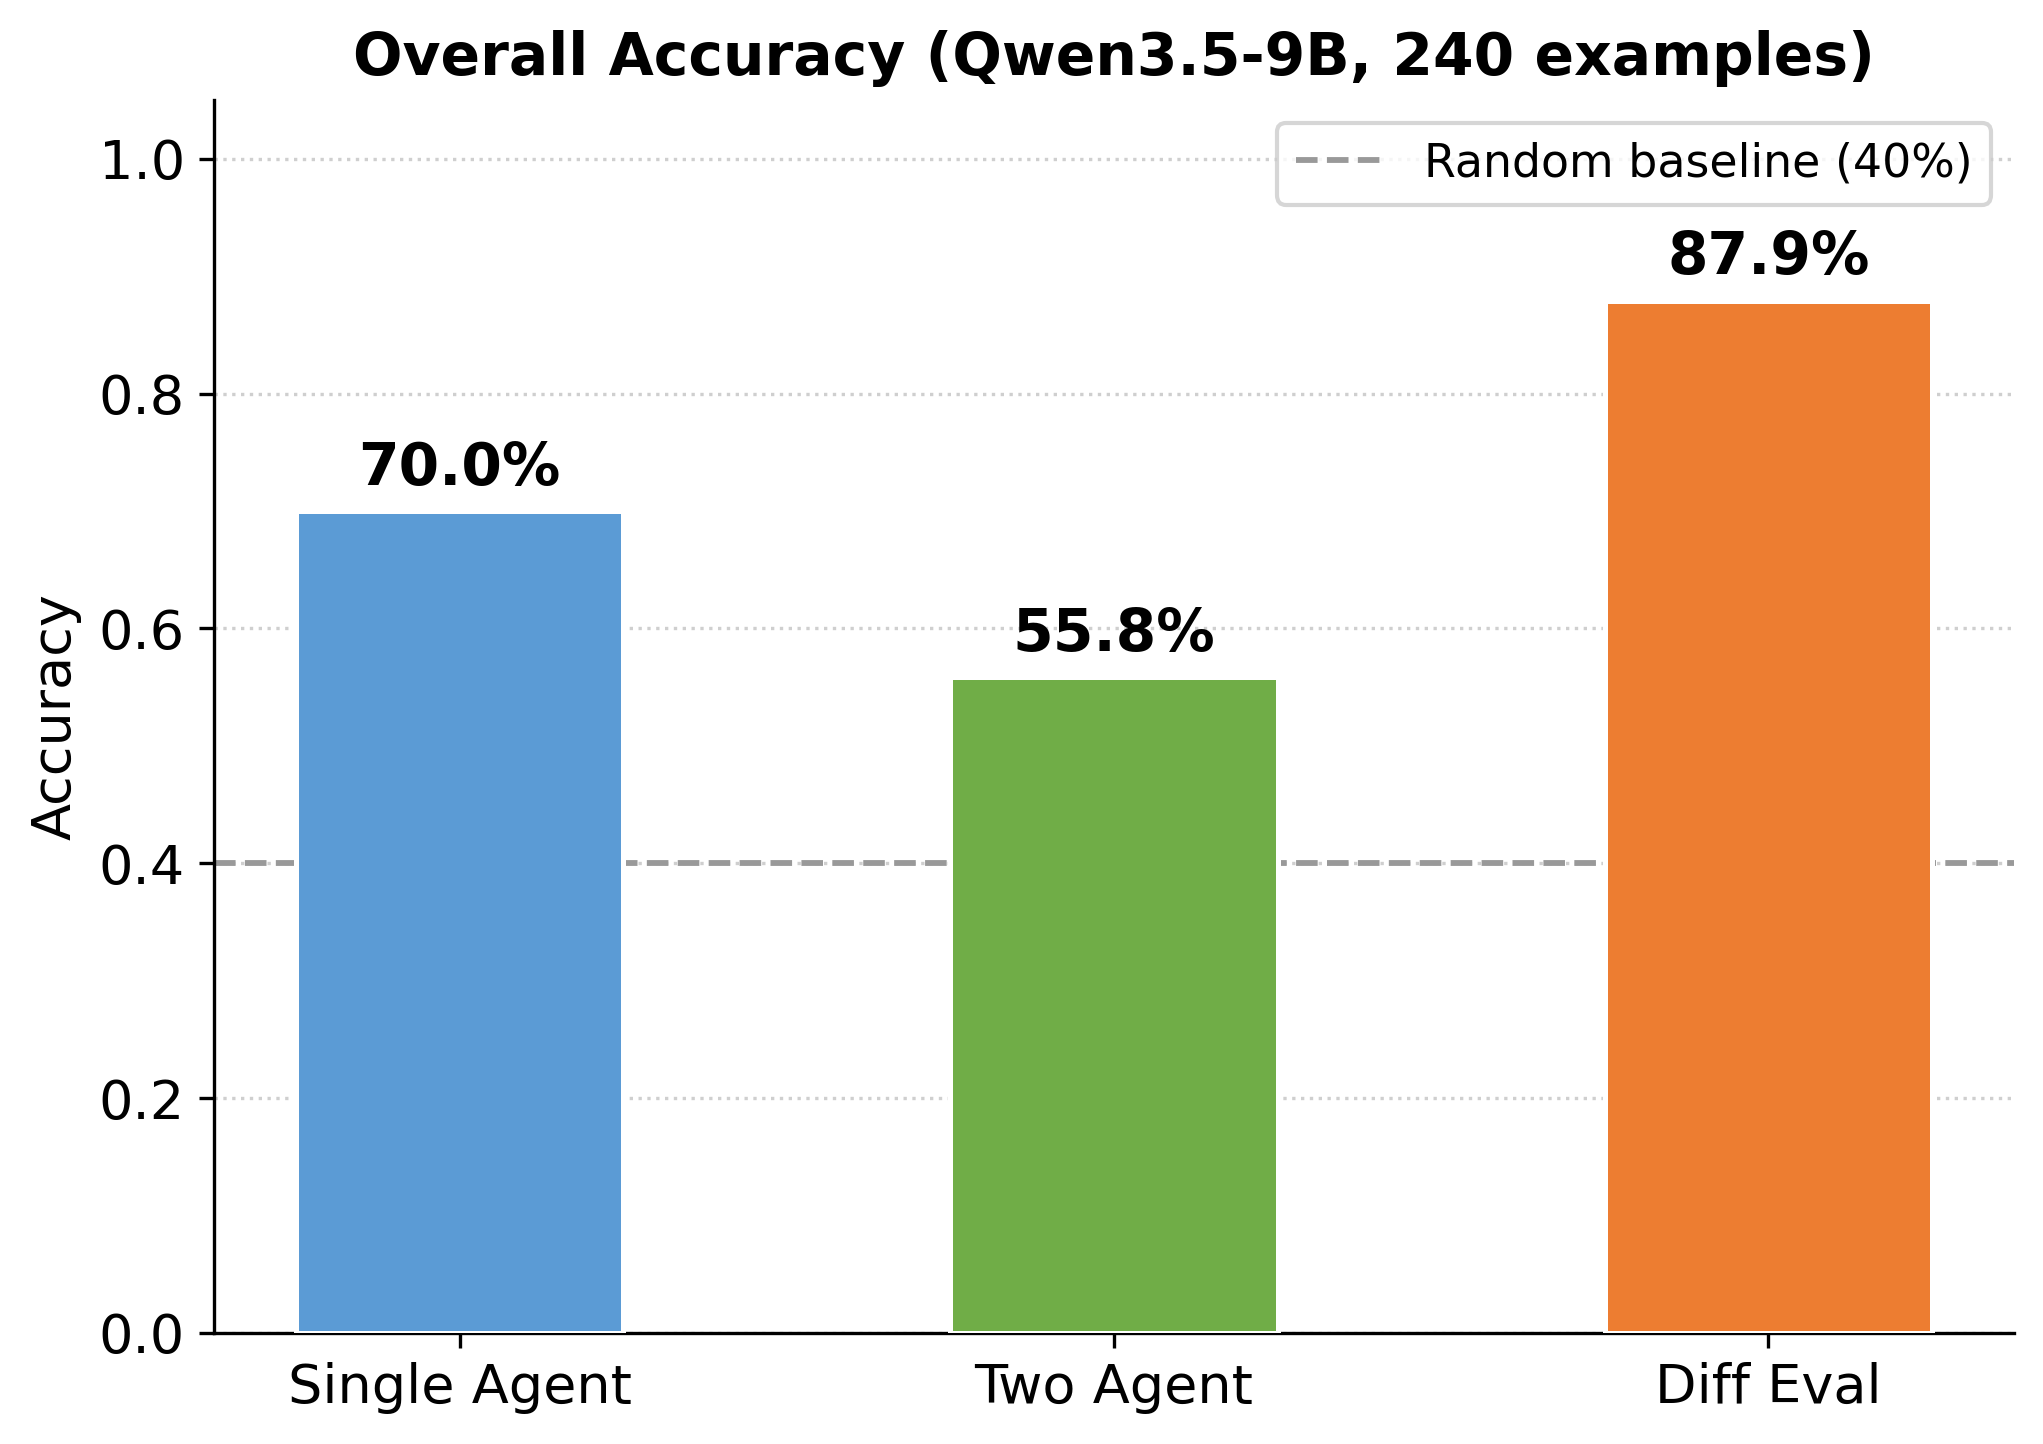
\includegraphics[width=0.85\textwidth]{paper_fig_overall.png}
\caption{Overall accuracy comparison across the three workflow methods.}
\label{fig:overall_accuracy}
\end{figure}

\section{Accuracy by SOLID Principle}

Table~\ref{tbl:by_principle} breaks down accuracy by SOLID principle, revealing striking differences in where each method excels.

\begin{table}[htbp]
\centering
\begin{tabular}{@{}lccc@{}}
\toprule
\textbf{Principle} & \textbf{Single Agent} & \textbf{Two-Agent} & \textbf{Diff Eval} \\
\midrule
SRP & 81.25\% & 87.50\% & \textbf{95.83\%} \\
OCP & \textbf{97.92\%} & 81.25\% & 72.92\% \\
LSP & 66.67\% & 33.33\% & \textbf{81.25\%} \\
ISP & 83.33\% & 37.50\% & \textbf{97.92\%} \\
DIP & 20.83\% & 39.58\% & \textbf{91.67\%} \\
\bottomrule
\end{tabular}
\caption{Top-2 accuracy by SOLID principle (48 examples each).}
\label{tbl:by_principle}
\end{table}

\begin{figure}[htbp]
\centering
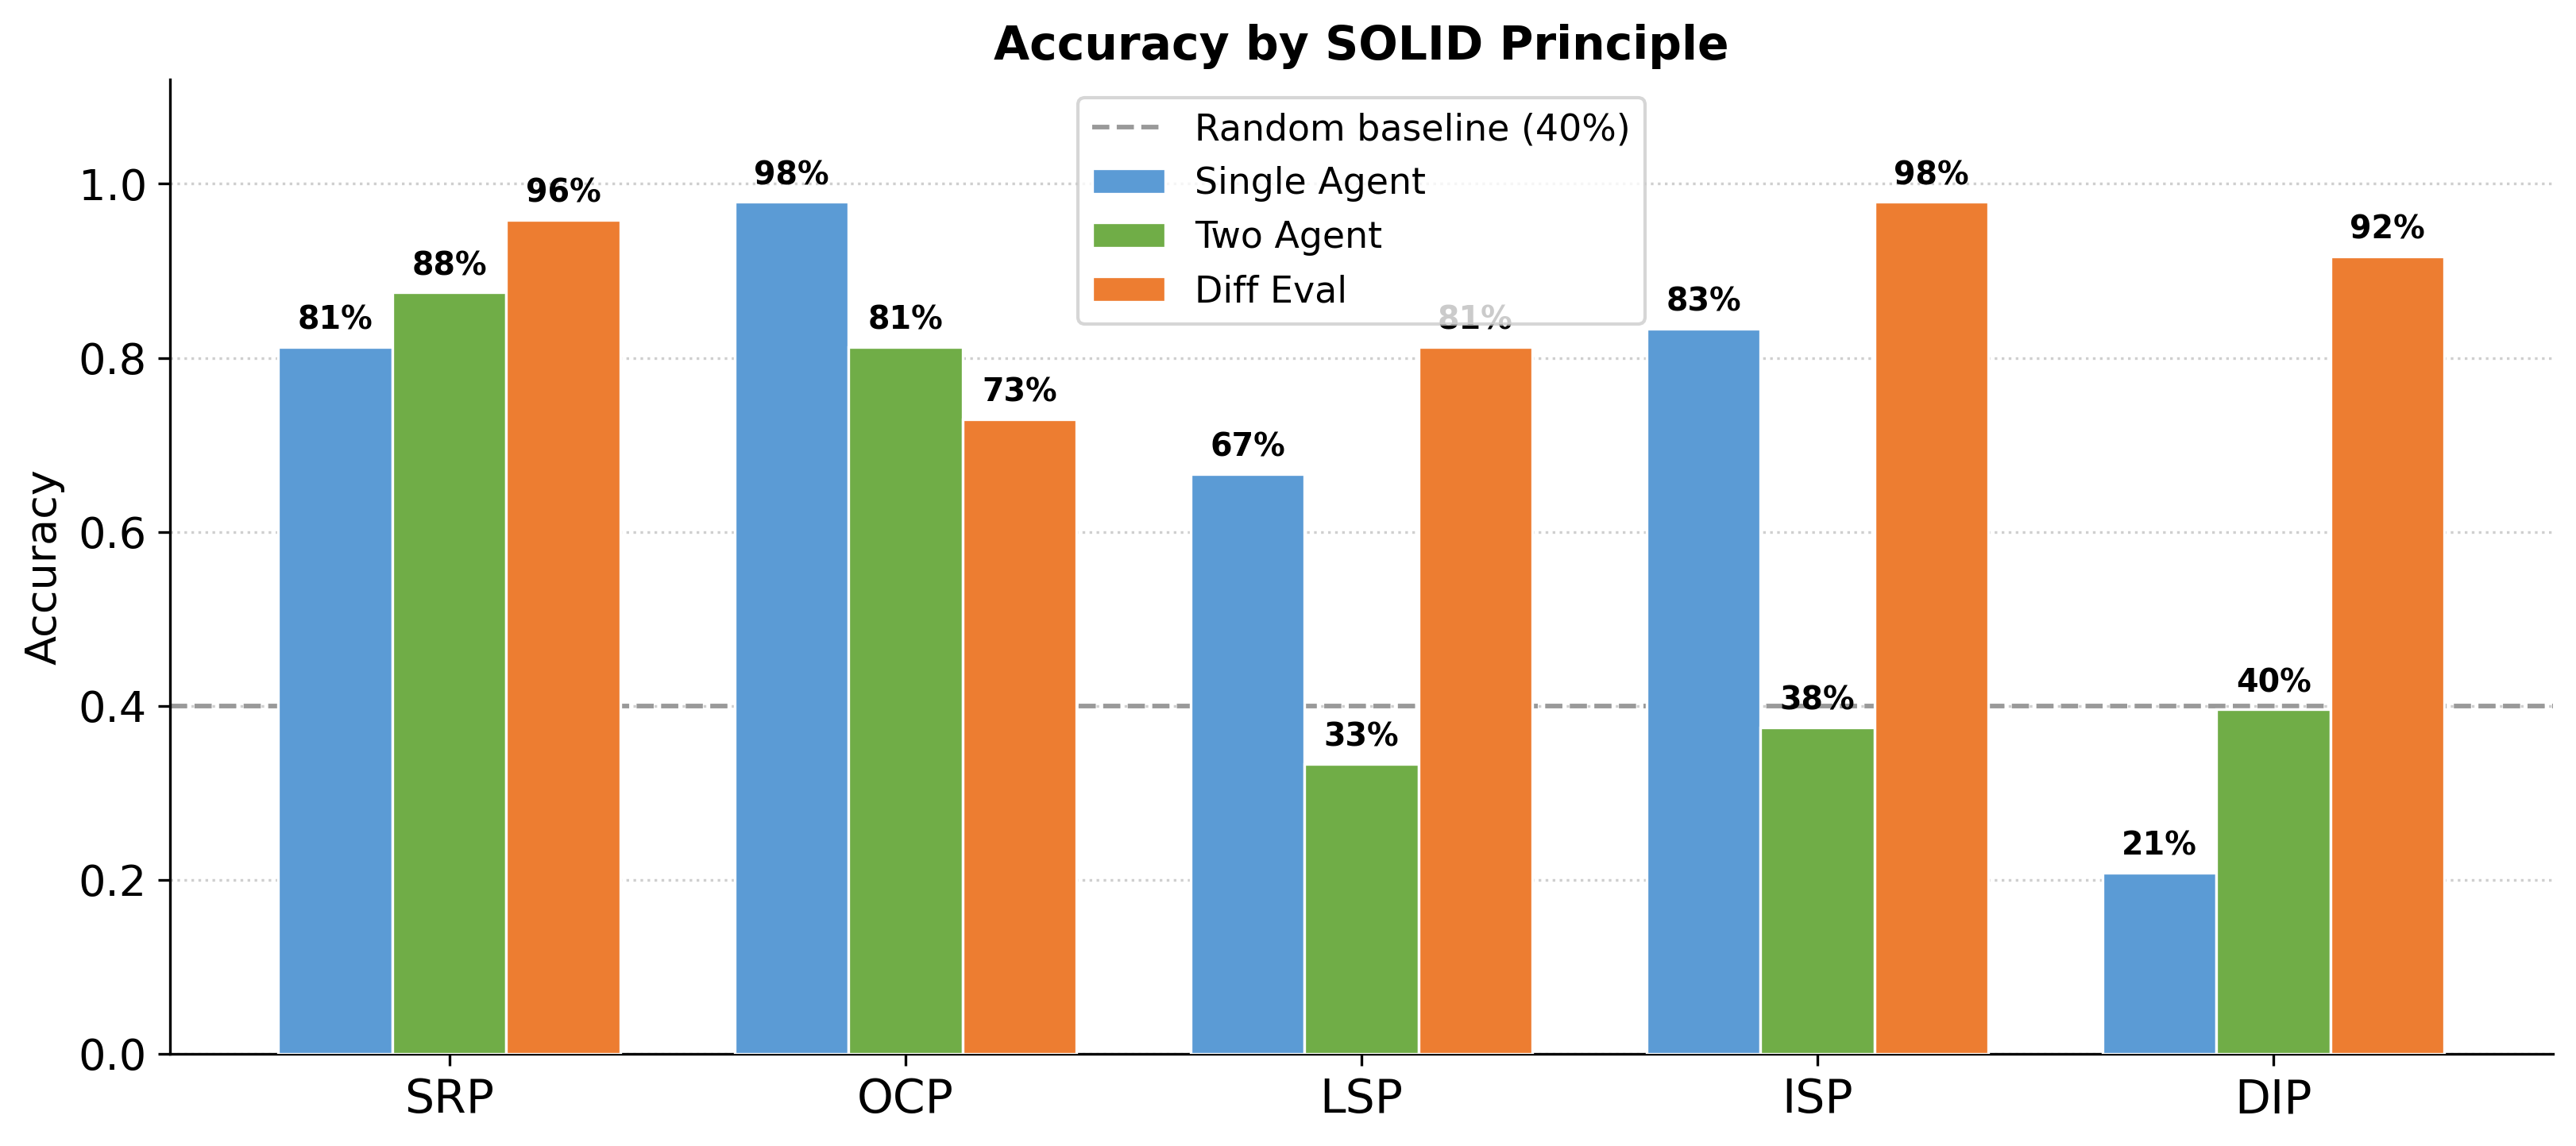
\includegraphics[width=0.85\textwidth]{paper_fig_violation.png}
\caption{Accuracy comparison by SOLID principle across the three methods.}
\label{fig:by_principle}
\end{figure}

Diff Eval leads on four of five principles. Single Agent retains an advantage only on OCP (97.92\% vs.\ 72.92\%), where rule-based pattern recognition of missing polymorphism is effective without requiring scenario simulation. For the structurally deep principles---DIP (91.67\%), ISP (97.92\%), and LSP (81.25\%)---Diff Eval's diff signal makes abstract violations concretely observable, delivering large gains over both baselines. Single Agent struggles particularly on DIP (20.83\%), reflecting that tight coupling is abstract until the code is forced to change.

\section{Accuracy by Difficulty Level}

Table~\ref{tbl:by_difficulty} shows performance across three difficulty levels, defined by code length.

\begin{table}[htbp]
\centering
\begin{tabular}{@{}lccc@{}}
\toprule
\textbf{Difficulty} & \textbf{Single Agent} & \textbf{Two-Agent} & \textbf{Diff Eval} \\
\midrule
Easy ($\sim$33 LOC)     & 75.00\% & 60.00\% & \textbf{92.50\%} \\
Moderate ($\sim$140 LOC) & 71.25\% & 62.50\% & \textbf{91.25\%} \\
Hard ($\sim$306 LOC)     & 63.75\% & 45.00\% & \textbf{80.00\%} \\
\bottomrule
\end{tabular}
\caption{Accuracy by difficulty level (80 examples each). Difficulty is determined by the number of lines of code.}
\label{tbl:by_difficulty}
\end{table}

\begin{figure}[htbp]
\centering
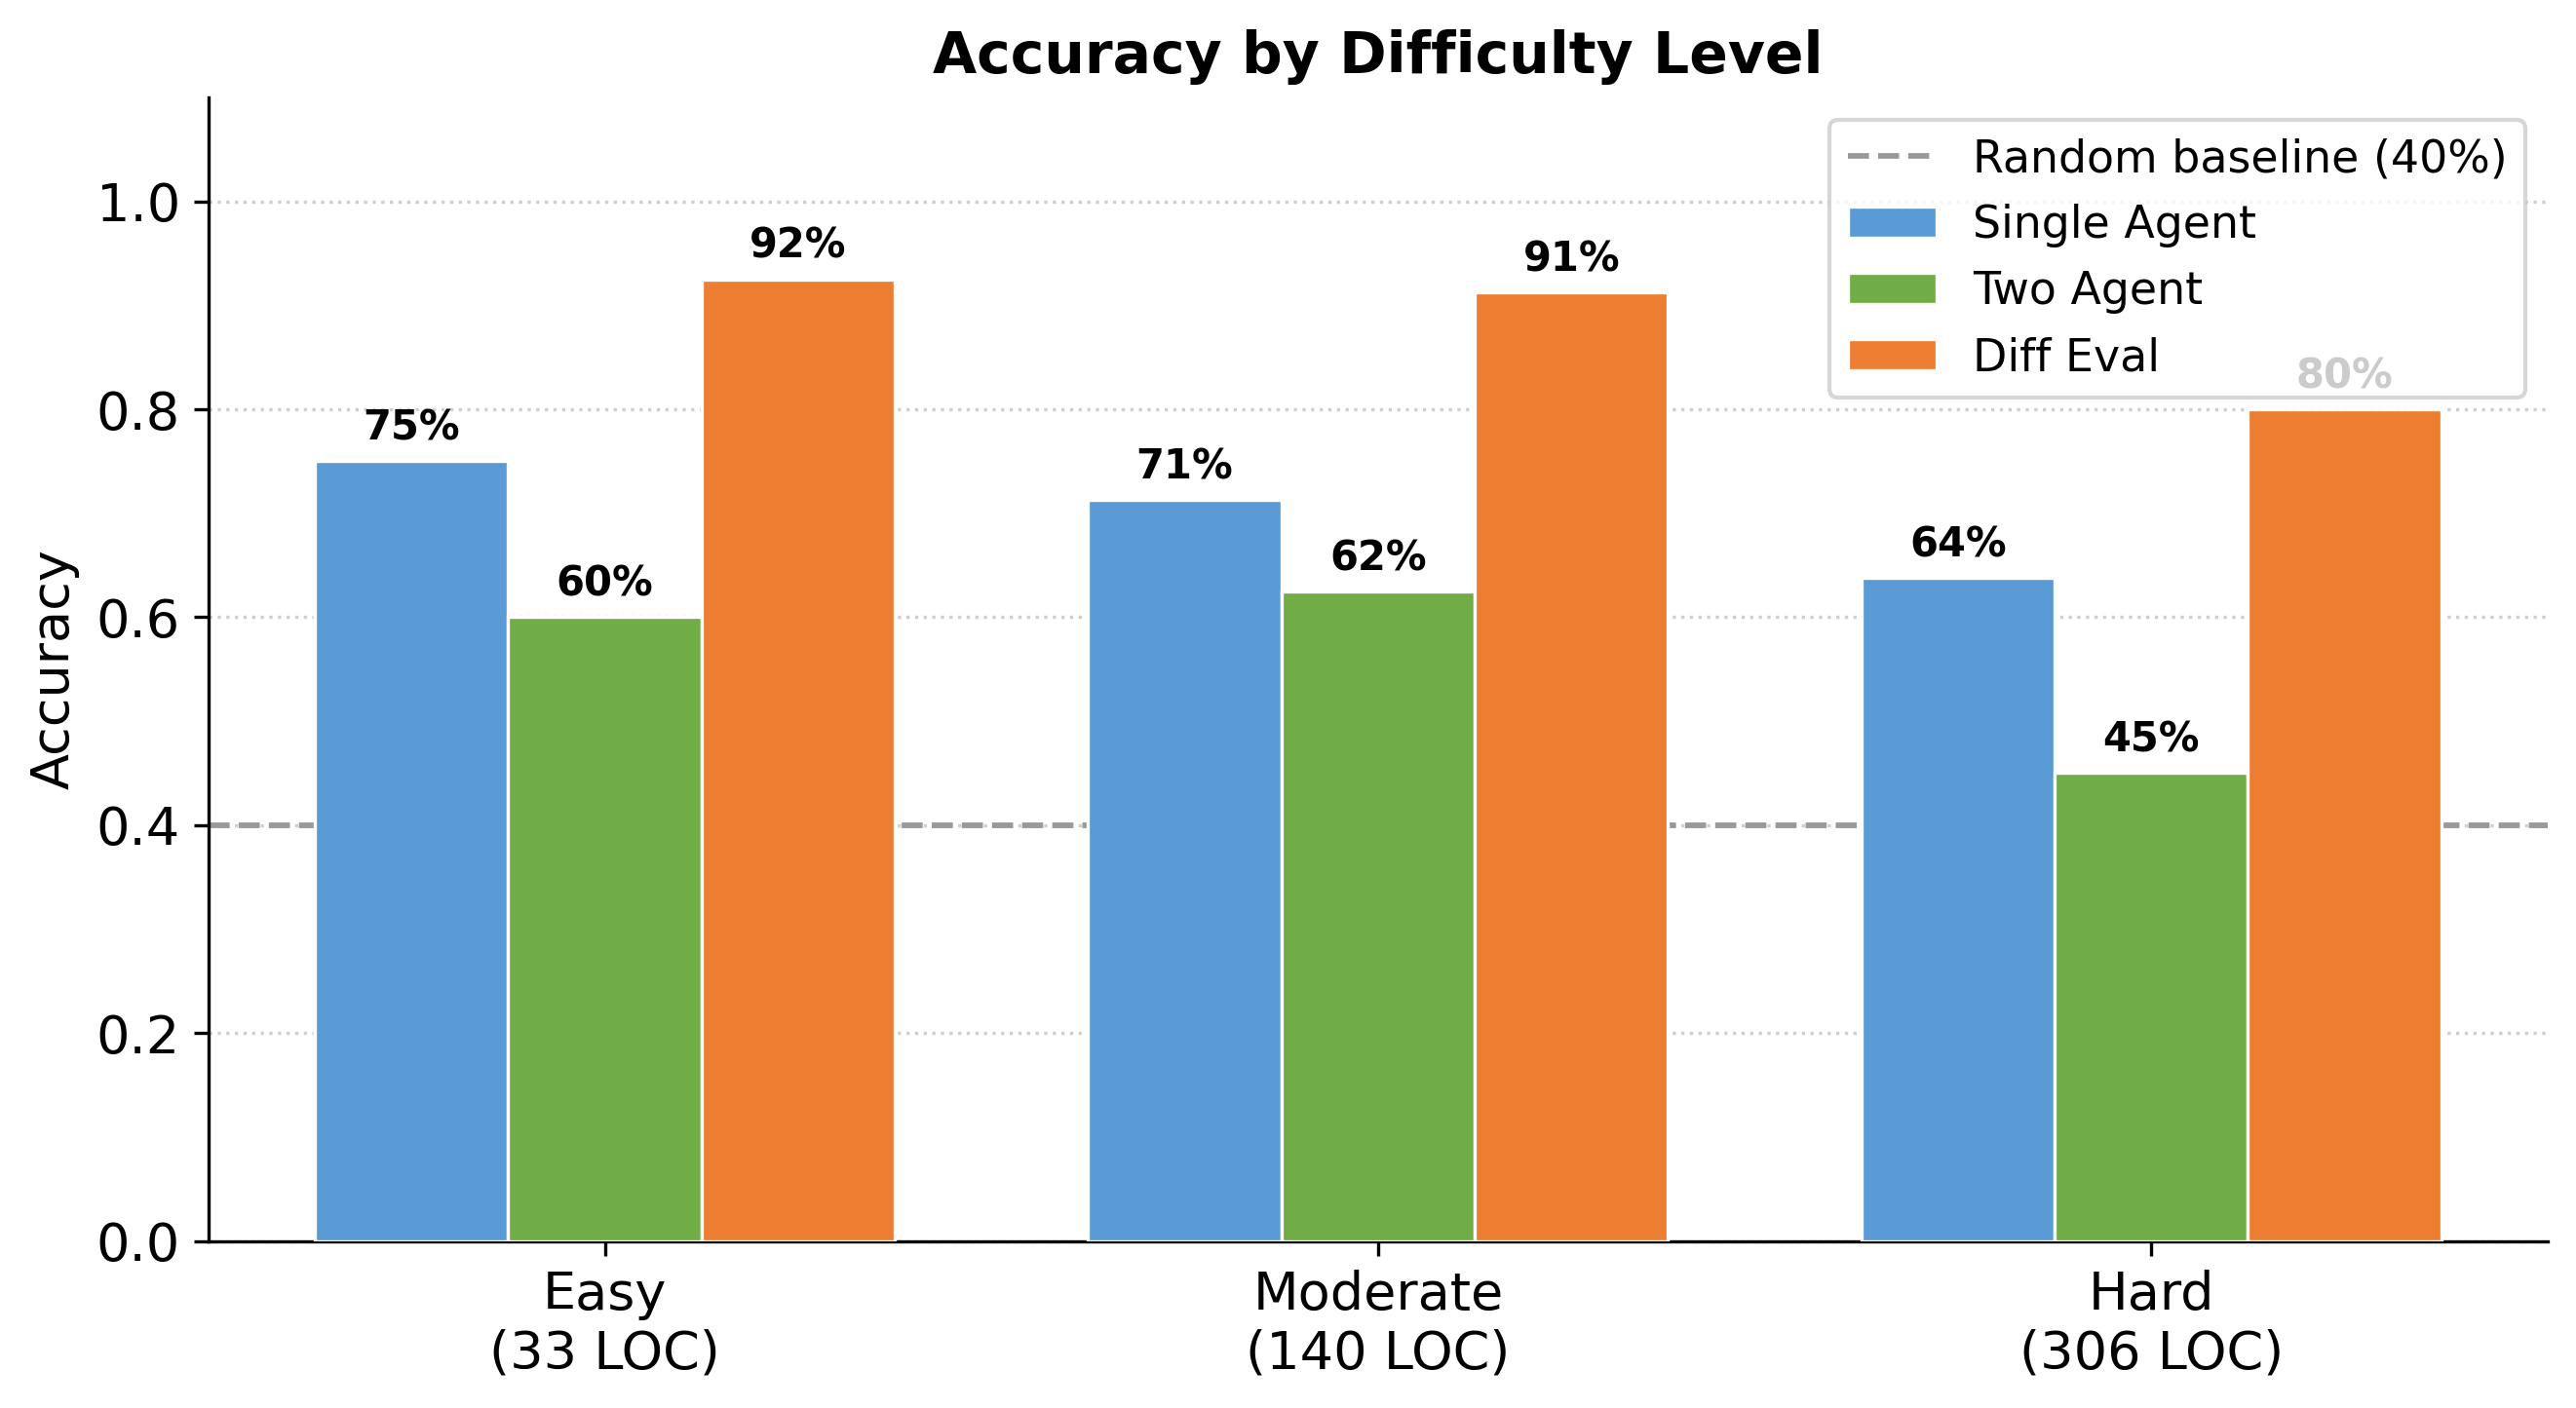
\includegraphics[width=0.85\textwidth]{paper_fig_difficulty.png}
\caption{Top-2 accuracy comparison by difficulty level across the three methods.}
\label{fig:by_difficulty}
\end{figure}

Diff Eval leads at every difficulty level and degrades the least with increasing code length: its drop from Easy to Hard is 12.5 pp (92.50\% $\to$ 80.00\%), compared to 11.25 pp for Single Agent (75.00\% $\to$ 63.75\%) and 15 pp for Two-Agent (60.00\% $\to$ 45.00\%). Critically, Diff Eval maintains 80.00\% even on Hard examples, whereas the baselines fall to 63.75\% and 45.00\% respectively, showing a sustained accuracy advantage of 16--35 pp on the most challenging inputs.

This robustness is attributable to the Pre-Verification stage in each detection channel. The pre-verifier receives only the \emph{diff} and the \emph{principle-specific signal mapping}---not the full original code. This effectively compresses the context: regardless of whether the original code is 33 or 306 lines, the diff highlights only the relevant changes. The Unified Ranking node therefore operates on pre-digested, principle-specific evidence rather than raw code, insulating it from the noise introduced by increasing lines of code.

\section{Comparison with Full-Size LLM}
\label{sec:vs_fullsize}

We evaluate \textbf{Qwen3.5 Plus}~\cite{Qwen2025} (released 2026-02-15)---the state-of-the-art closed-source model from the Qwen family as of March 2026---using the identical Single Agent prompt, isolating workflow design as the sole variable.

\begin{table}[htbp]
\centering
\begin{tabular}{@{}lcc@{}}
\toprule
\textbf{System} & \textbf{Top-2 Acc.} & \textbf{MRR@2} \\
\midrule
Qwen3.5 9B --- Single Agent (local) & 70.00\% & 0.638 \\
\textbf{Qwen3.5 9B --- Diff Eval (local)} & \textbf{87.92\%} & \textbf{0.792} \\
\midrule
Qwen3.5 Plus --- Single Agent (cloud) & 95.83\% & 0.858 \\
\bottomrule
\end{tabular}
\caption{Qwen3.5 9B workflows vs.\ Qwen3.5 Plus (cloud). Diff Eval closes $\sim$70\% of the performance gap through workflow design alone.}
\label{tbl:vs_fullsize}
\end{table}

The plain 9B baseline lags the full-size model by 25.83 pp; Diff Eval recovers 17.92 pp of that gap without any increase in model size or cloud dependency, demonstrating that \textbf{workflow design is a primary lever for closing the capability gap between local and cloud-scale models}.


% ============================================================
\chapter{Discussion}
\label{ch:discussion}
% ============================================================

\section{Error Analysis}

Figure~\ref{fig:confusion_matrix} shows the Top-2 resolved confusion matrix for Diff Eval. The dominant off-diagonal cluster is \textbf{SRP over-prediction}: OCP$\to$SRP (11 cases), LSP$\to$SRP (5), and DIP$\to$SRP (3) account for 19 of the 29 errors. Responsibility-mixing symptoms arise in many violation types---an OCP violation forcing edits across methods, or a DIP violation adding cross-cutting concerns, can resemble SRP at the diff level, suggesting the Unified Ranking step would benefit from a penalty for over-frequent SRP selection. LSP is the noisiest category (scatter to SRP and DIP), while ISP and SRP themselves are near-perfect (47/48 and 46/48).

\begin{figure}[htbp]
\centering

\includegraphics[width=0.72\textwidth]{paper_fig_confusion.png}
\caption{Top-2 resolved confusion matrix for Diff Eval. Dominant error: SRP over-prediction (19 off-diagonal cases).}
\label{fig:confusion_matrix}
\end{figure}

\section{Why Diff Eval Works}

Diff Eval converts an abstract judgment (``is this code SOLID?'') into a concrete, observable task (``what changed in the diff?''). This grounds detection in objective structural evidence rather than subjective LLM assessment, applies principle-specific probing that surfaces violations under exactly the conditions where they manifest, and decomposes a complex judgment into simpler, verifiable pipeline stages.

\textbf{DIP and ISP} benefit most: these principles are inherently about dependencies and interfaces---invisible in a static snapshot but concrete when code is forced to accommodate a change. Diff Eval reaches 91.67\% on DIP (\emph{matching Qwen3.5 Plus}) and 97.92\% on ISP, against 20.83\% and 83.33\% for Single Agent. \textbf{OCP} is the exception: its surface-visible \texttt{if-else}/\texttt{switch} pattern is better captured by direct inspection, explaining the 97.92\% vs.\ 72.92\% gap in favour of Single Agent. \textbf{Hard examples} favour Diff Eval (80.00\% vs.\ 63.75\% SA / 45.00\% TA) because Pre-Verification receives only the compact diff, not the full source.

\section{Privacy and Observability}

Enterprise and government codebases frequently contain regulated or proprietary data that cannot be sent to external APIs without violating compliance requirements---including the EU AI Act~\cite{EUAIAct2024}, Katakri 2020~\cite{Katakri2020}, and broader cloud privacy concerns documented in the literature~\cite{Ghorbel2017}. Diff Eval runs entirely on consumer hardware (RTX 4060 8GB) via Ollama~\cite{Ollama2024} with \textbf{zero data egress}, achieving 87.92\% accuracy while closing 70\% of the gap to cloud-scale inference.

Beyond privacy, Diff Eval is fully \textbf{observable}: every intermediate artifact---scenario description, modified code, diff, per-principle verdicts, and ranking rationale---is persisted and inspectable. Developers can trace any verdict back to the specific diff that produced it, turning the tool from a black-box classifier into a transparent reasoning chain that supports productive disagreement rather than blind acceptance.

\section{Limitations}

\begin{itemize}
  \item \textbf{OCP accuracy}: Diff Eval's weakest result is OCP (72.92\%). The root cause is scenario cross-contamination: the SRP extension scenario is broad enough to absorb OCP violation signals, causing SRP to rank first. This reflects a deeper ambiguity in SOLID itself---``responsibility'' and ``extension'' are notoriously ill-defined, and their conceptual overlap is a structural property of the taxonomy. Pehlivan et al.~\cite{Pehlivan2025} observe the same pattern: DIP violations are disproportionately misclassified as SRP or OCP, confirming the issue is not model-specific.
  \item \textbf{Runtime cost}: 20 inference calls per example (mean 151.6s) versus 1 call for Single Agent (2.1s). Offset by local execution and GPU-level parallelism potential.
  \item \textbf{Dataset scope}: The 240-example benchmark is relatively small; larger-scale evaluation would strengthen the findings.
\end{itemize}

% ============================================================
\chapter{Conclusions}
\label{ch:conclusions}
% ============================================================

This work demonstrates a core principle: \textbf{Small LLM + Agentic Workflow $\approx$ Full-Size LLM, in the code quality detection scenario}. The Diff Eval approach---testing code by attempting to extend it and observing the resulting diff---achieves 87.92\% accuracy on SOLID principle violation detection using a local 9B model, closing approximately 70\% of the performance gap to a full-size cloud LLM (Qwen3.5 Plus, 95.83\%) that uses the identical single-agent prompt. The plain small-model baseline achieves only 70.00\%; Diff Eval recovers 17.92 of the 25.83 pp deficit through workflow design alone, with zero increase in model size and zero data egress.

The key insight is that design quality is better revealed through \textbf{behavioral observation} (\textbf{what happens when you try to change the code}) than through \emph{static judgment} (does this code look right)---a process that mirrors how developers actually reason about code quality during real-world software development. This principle---converting abstract reasoning into concrete, observable evidence---may generalize beyond SOLID detection to other areas of software quality assessment.

Future work includes: (1) a hybrid approach combining the best method per principle, (2) improved OCP scenario generation, (3) larger-scale evaluation with diverse codebases, and (4) integration into continuous integration pipelines for real-time code review.

% ============================================================
% References
% ============================================================
\chapter*{References}
\label{references}
\addcontentsline{toc}{chapter}{References}

\printbibliography[heading=none]


\end{document}
